\documentclass[aspectratio=169]{beamer}
\usepackage{math214}
\usepackage{babel}

%\usepackage{enumitem}
% Then, after \begin{document}, you can begin your frames/slides

\title{\LARGE 255RC6}
\author{Shi Chengyang, Deng Ruizhi, Shen Haoran, Tang Jingfan}
\date{Summer 2025}

\definecolor{darkblue}{HTML}{6666dd} 
\colortheme{green!30!black}
%\colortheme{orange!85!black}
%\colortheme{darkblue}
%\colortheme{blue!100!black}
%\colortheme{orange!85!white!90!black}
\begin{document}

\maketitle

%\begin{frame}
 %  \frametitle{}
  %  \tableofcontents     % 生成目录
%\end{frame}


\begin{frame}{Contents}
    \begin{enumerate}
        \item \hyperlink{1}{Curl and Divergence}
        \item \hyperlink{2}{Parametric Surfaces and Areas}
        \item \hyperlink{3}{Surface Integrals}
    \end{enumerate}
       
\end{frame}

    

\section{Curl and Divergence}
\begin{frame}{Curl}

    \begin{block}{Definition}
$\boldsymbol{F}=P\boldsymbol{i}+Q\boldsymbol{j}+R\boldsymbol{k}$ is a vector field on $\mathbb{R}^3$ and the partial derivatives of $P$,$Q$, and $R$ all exist, then the $\boldsymbol{curl}$ of $\boldsymbol{F}$ is the vector field on defined by
    \begin{align*}
        \nabla\times \boldsymbol{F} = &
        \left|
        \begin{array}{ccc}
            \boldsymbol{i}& \boldsymbol{j}& \boldsymbol{k}\\
            \frac{\partial}{\partial x}& \frac{\partial}{\partial y}&\frac{\partial}{\partial z}\\
            P&Q&R
        \end{array}
        \right| \\
        =& (\frac{\partial R}{\partial y}-\frac{\partial Q}{\partial z})\boldsymbol{i}+(\frac{\partial P}{\partial z}-\frac{\partial R}{\partial x})\boldsymbol{j}+(\frac{\partial Q}{\partial x}-\frac{\partial P}{\partial y})\boldsymbol{k}\\
        =&\text{curl } \boldsymbol{F}
    \end{align*}
    \end{block}

    \begin{block}{Theorem}
        If $f$ is a function of three variables that has continuous second-order partial derivatives, then
        \begin{equation*}
            curl(\nabla f)=\boldsymbol{0}
        \end{equation*}
    \end{block}
\end{frame}

\begin{frame}{Divergence}
    \begin{block}{Definition}
        $\boldsymbol{F}=P\boldsymbol{i}+Q\boldsymbol{j}+R\boldsymbol{k}$ is a vector field on $\mathbb{R}^3$ and $\partial P/\partial x$,$\partial Q/\partial y$, and $\partial R/\partial z$ exist, then the $\boldsymbol{divergence}$ of $\boldsymbol{F}$ is the  function of three variables defined by
        \begin{equation*}
            \nabla \cdot \boldsymbol{F} = \frac{\partial P}{\partial x}+\frac{\partial Q}{\partial y}+\frac{\partial R}{\partial z}
        \end{equation*}
    \end{block}

    \begin{block}{Theorem}
        If $\boldsymbol{F}=P\boldsymbol{i}+Q\boldsymbol{j}+R\boldsymbol{k}$ is a vector field on $\mathbb{R}^3$ and $P$, $Q$ , and $R$ have continuous second-order partial derivatives, then
        \begin{equation*}
        \text{div curl }\boldsymbol{F}=0
        \end{equation*}
    \end{block}
\end{frame}

\begin{frame}{Exercises}
    \textbf{Ex 8.1} Vector field $\boldsymbol{F}=(x^2y,y^2z,z^2x)$, evaluate the divergence of  the vector field at point (2,1,-2).\\
    \par
    \textbf{Ex 8.2} Given a rigid body rotating about the z-axis with angular velocity $\boldsymbol{\omega}=(0,0,\omega)$, find the curl of the linear velocity $\boldsymbol{\nu}$ at any point M on the rigid body.\\
    \par
\end{frame}

\begin{frame}{Solutions}
    \textbf{Solution 8.1} -8\\
    \par
    \textbf{Solution 8.2} $\nabla\times \boldsymbol{\nu}=2\boldsymbol{w}$
\end{frame}

\begin{frame}{Exercises}
    \textbf{Ex 8.3} Prove the following identities. Assuming that the appropriate partial derivatives exist and are continuous. $f$ is a scalar field and $\boldsymbol{F}$, $\boldsymbol{G}$ are vector fields.\\
    \begin{enumerate}
        \item div($f\boldsymbol{F}$)=$f$ div $\boldsymbol{F}$+$\boldsymbol{F}\cdot \nabla f$
         \item curl($f\boldsymbol{F}$)=$f$ curl $\boldsymbol{F}$+$(\nabla f)\times\boldsymbol{F}$
         \item div($\boldsymbol{F}\times\boldsymbol{G}$)=$\boldsymbol{G}\cdot$ curl $\boldsymbol{F}$-$\boldsymbol{F}\cdot$ curl $\boldsymbol{G}$
    \end{enumerate}
    
\end{frame}

\begin{frame}{Solution}
    If $f$ is a scalar field and $\boldsymbol{F}$, $\boldsymbol{G}$ are vector fields, then $f\boldsymbol{F}$,$\boldsymbol{F}\cdot\boldsymbol{G}$, and $\boldsymbol{F}\times\boldsymbol{G}$ are defined by
    \begin{align*}
        (f\boldsymbol{F})(x,y,z)&=f(x,y,z)\boldsymbol{F}(x,y,z)\\
        (\boldsymbol{F}\cdot\boldsymbol{G})(x,y,z)&=\boldsymbol{F}(x,y,z)\cdot\boldsymbol{G}(x,y,z)\\
        (\boldsymbol{F}\times\boldsymbol{G})(x,y,z)&=\boldsymbol{F}(x,y,z)\times\boldsymbol{G}(x,y,z)
    \end{align*}
\end{frame}

\section{Parametric Surfaces and Areas}

\begin{frame}{Parametric Surfaces}
    \begin{block}{Definition}
        We suppose that 
        \begin{equation*}
            \boldsymbol{r}(u,v)=x(u,v)\boldsymbol{i}+y(u,v)\boldsymbol{j}+z(u,v)\boldsymbol{k}
        \end{equation*}
        is a vector-valued function defined on a region $D$ in the $uv$-plane. The set of all points (x,y,z) in $\mathbb{R}^3$ is called a \textbf{parametric surface} $S$. Equations
        \begin{equation*}
            x=x(u,v)\qquad y=y(u,v) \qquad z=z(u,v)
        \end{equation*}
        .are called \textbf{parametric equations} of $S$.
    \end{block}
\end{frame}


\begin{frame}{Surface Areas}
    \begin{block}{Definition}
        If a smooth parametric surface $S$ is given by the equation
         \begin{equation*}
            \boldsymbol{r}(u,v)=x(u,v)\boldsymbol{i}+y(u,v)\boldsymbol{j}+z(u,v)\boldsymbol{k} \qquad (u,v)\in D
        \end{equation*}
        and $S$ is covered just once as $(u,v)$ ranges throughout the parameter domain $D$, then the \textbf{surface area} of $S$ is
        \begin{equation*}
            A=\iint_D \big|\boldsymbol{r}_u\times\boldsymbol{r}_v\big|dA
        \end{equation*}
        where
        \begin{equation*}
            \boldsymbol{r}_u=\frac{\partial x}{\partial u}\boldsymbol{i}+\frac{\partial y}{\partial u}\boldsymbol{j}+\frac{\partial z}{\partial u}\boldsymbol{k} \quad \qquad \boldsymbol{r}_v=\frac{\partial x}{\partial v}\boldsymbol{i}+\frac{\partial y}{\partial v}\boldsymbol{j}+\frac{\partial z}{\partial v}\boldsymbol{k}
        \end{equation*}
    \end{block}
\end{frame}

\begin{frame}
    \frametitle{Spacial Case}
    \begin{block}
        If the surface can be expressed with equation $z=f(x,y)$, let $u=x,v=y$, we have
        \begin{equation*}
            x=x \qquad y=y \qquad z=f(x,y)
        \end{equation*}
        then
        \begin{equation*}
            \boldsymbol{r}_x=\boldsymbol{i}+(\frac{\partial f}{\partial x})\boldsymbol{k} \qquad \qquad \boldsymbol{r}_y=\boldsymbol{j}+(\frac{\partial f}{\partial y})\boldsymbol{k}
        \end{equation*}
        We have
        \begin{equation*}
            \big|\boldsymbol{r}_x\times\boldsymbol{r}_y\big|=\big|-\frac{\partial f}{\partial x}\boldsymbol{i}-\frac{\partial f}{\partial y}\boldsymbol{j}+\boldsymbol{k}\big|=\sqrt{1+(\frac{\partial z}{\partial x})^2+(\frac{\partial z}{\partial y})^2}
        \end{equation*}
    \end{block}
    
\end{frame}

\begin{frame}{Exercises}
    \textbf{Ex 8.4} Find the area of the following surfaces
    \begin{itemize}
        \item The part of the plane $3x+2y+z=6$ that lies in the first octant.
        \item The helicoid (or spiral ramp) with vector equation $\boldsymbol{r}(u,v)=u\cos{v}\boldsymbol{i}+u\sin{v}\boldsymbol{j}+v\boldsymbol{k},0\leq u\leq 1,0\leq v\leq\pi$
    \end{itemize}
    
\end{frame}

\begin{frame}{Solutions}
\textbf{Solution 8.4}
\begin{itemize}
    \item $3\sqrt{14}$
    \item $\frac{\pi}{2}[\sqrt{2}+ln(1+\sqrt{2})]$
\end{itemize}
    
\end{frame}

\section{Surface Integrals}

\begin{frame}{Surface Integrals}
    \begin{block}{Types}
        \begin{enumerate}
            \item surface integral of $f$ over the surface $S$
            \begin{equation*}
                \iint_Sf(x,y,z)dS=\iint_D f(\boldsymbol{r}(u,v))\big|\boldsymbol{r}_U\times\boldsymbol{r}_v\big|dA
            \end{equation*}
            \item surface integral of $\boldsymbol{F}$ over an oriented surface $S$ is
            \begin{equation*}
                \iint_S \boldsymbol{F}\cdot d\boldsymbol{S}=\iint_S \boldsymbol{F}\cdot\boldsymbol{n}dS
            \end{equation*}
            This integral is also called the \textbf{flux} of $\boldsymbol{F}$ across $S$.
        \end{enumerate}
        
    \end{block}
    
\end{frame}
\begin{frame}{Surface Integrals}
    \frametitle{urface Integrals}
    \begin{block}{Oriented Surface Integral}
        Suppose the surface is parametrized by $r(u,v)$ and the unit normal is given by $\hat{n} = \frac{r_u \times r_v}{||r_u \times r_v||}$.

    Then $\iint_S F \cdot dS = \iint_S (F \cdot \hat{n}) \,d\sigma$
    $= \iint_D F \cdot \frac{r_u \times r_v}{||r_u \times r_v||} ||r_u \times r_v|| \,dA$
    $= \iint_D F \cdot (r_u \times r_v) \,dA$.
    \end{block}
\end{frame}
\begin{frame}{Exercises}
\textbf{Ex 8.5} Evaluate the following surface integrals.
    \begin{enumerate}
    \item
Calculate the surface integral
\[
\iint_S (x + y^2) \, dS,
\]
where \( S \) is the surface of the cylinder given by \( x^2 + y^2 = 4 \) and \( 0 \leq z \leq 3 \).
\item 
Calculate the surface integral:
\[
\iint_S (x^2 - z) \, dS,
\]
where \( S \) is the surface with parameterization
\[
\mathbf{r}(u,v) = \langle v, u^2 + v^2, 1 \rangle, \quad 0 \leq u \leq 2, \quad 0 \leq v \leq 3.
\]

\end{enumerate}
\end{frame}

\begin{frame}{Exercises}
    \frametitle{Exercises}
    \begin{enumerate}
        \item $\mathbf{F}(x, y, z) = xy\,\mathbf{i} + 4x^2\,\mathbf{j} + yz\,\mathbf{k}, \quad S \text{ is the surface } z = xe^y, \quad 0 \le x \le 1, 0 \le y \le 1, \text{ with upward orientation}$
        \item $\mathbf{F}(x, y, z) = xz\,\mathbf{i} + x\,\mathbf{j} + y\,\mathbf{k}, \quad S \text{ is the hemisphere } x^2 + y^2 + z^2 = 25, y \ge 0, \text{ oriented in the direction of the positive y-axis}$
    \end{enumerate}
\end{frame}

\begin{frame}{Answers}
    \begin{enumerate}
        \item $24 \pi$
        \item $24$
    \end{enumerate}
\end{frame}

\begin{frame}{Answers}
    $\mathbf{F}(x, y, z) = xy\,\mathbf{i} + 4x^2\,\mathbf{j} + yz\,\mathbf{k}, \quad z = g(x, y) = xe^y, \text{ and } D \text{ is the square } [0, 1] \times [0, 1], \text{ so by Equation 10}$
                \begin{align*}
                    \iint_S \mathbf{F} \cdot d\mathbf{S} &= \iint_D [-xy(e^y) - 4x^2(xe^y) + yz] \, dA \\
                    &= \int_0^1 \int_0^1 (-xye^y - 4x^3 e^y + xye^y) \, dy \, dx \\
                    &= \int_0^1 \left[-4x^3 e^y\right]_{y=0}^{y=1} \, dx = (e-1) \int_0^1 (-4x^3) \, dx = 1-e
                \end{align*}
\end{frame}

\begin{frame}{Answers}
   \begin{figure}
            \centering
            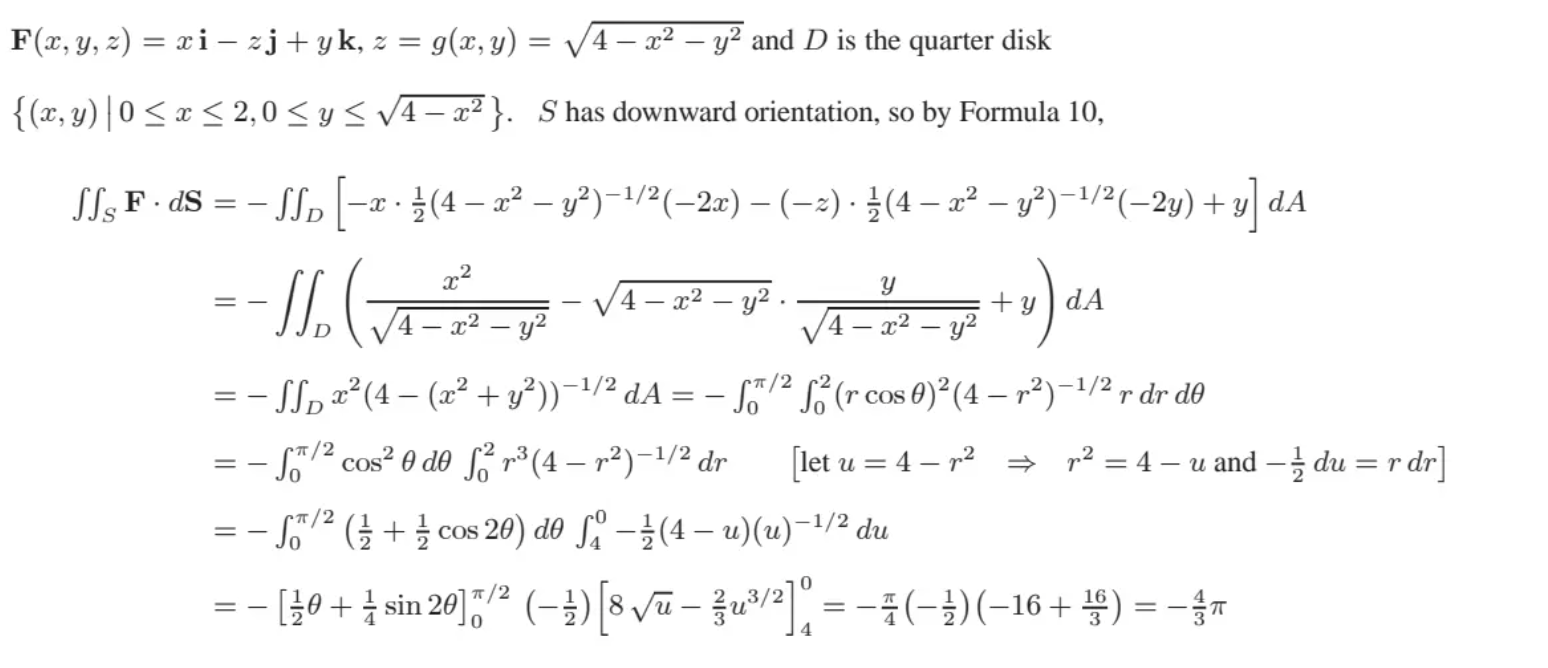
\includegraphics[width=1\linewidth]{ans.png}
            \label{fig:enter-label}
        \end{figure}

\end{frame}

\begin{frame}{\textcolor{green!30!black}{end}}
    \begin{center}
        \LARGE Thank you!
    \end{center}
\end{frame}



\end{document}

